\documentclass[10pt,journal,draftclsnofoot,onecolumn]{IEEEtran}
\hyphenation{op-tical net-works semi-conduc-tor}

\usepackage[margin=.75in]{geometry}
\usepackage{courier}
\usepackage{ifthen}
\usepackage{setspace}
\usepackage{listings}
\usepackage[usenames, dvipsnames]{color}
\usepackage{tabularx}
\usepackage[strict]{chngpage}
\usepackage{cite}
\usepackage{graphicx}
\usepackage{acronym}
\usepackage{color}

\acrodef{OSU}[OSU]{Oregon State University}
\acrodef{AIAA}[AIAA]{American Institute of Aeronautics and Astronautics}
\acrodef{AGL}[AGL]{Above Ground Level}

\lstset {
	language=C,
	basicstyle=\ttfamily,
	keywordstyle=\color{blue}\ttfamily,
	stringstyle=\color{red}\ttfamily,
	commentstyle=\color{OliveGreen}\ttfamily,
	morecomment=[l][\color{magenta}]{\#}
	showstringspaces=false,
	showspaces=false,
	frame=single,
	captionpos=b
}

\newcommand{\commandline}[2][\empty] {
	\begin{quote}
		\texttt{#2}
		\ifthenelse{\equal{#1}{\empty}}{}{\begin{quote}#1\end{quote}}
	\end{quote}
}

\begin{document}
	\singlespace
	
	\title{\vspace{2in}Problem Statement}
	
	\author {
		Anisimova, Natasha
		\and
		Lee, Terrance
		\and
		Morgan, Albert
	}
	
	\markboth{CS Capstone 2016-2017}{Requirements}
	
	\pagestyle{empty}
	\vspace*{2in}
	\begin{center}
		\huge
		Requirements\\
		\normalsize
		\vspace{5mm}
		CS Capstone\\
		Spring 2016\\
		\vspace{5mm}
		Natasha Anisimova\\
		Terrance Lee\\
		Albert Morgan
	\end{center}
	
	\vspace{5mm}
	
	\begin{center}
		\textbf{Abstract}
	\end{center}
	
	\begin{adjustwidth}{2in}{2in}
	
	The \textit{Groundstation} software will collect telemetry from a rocket while it is in flight and graphically display the telemetry in real-time.
	Collecting the telemetry in real-time will reduce the chances of a failure-to-recover by allowing the ground team to track the rocket during its flight.
	The graphical display will make the telemetry instantly understandable without time-consuming analysis.
	This document will detail the specific requirements of the Groundstation software.

	
	\end{adjustwidth}
	
	\newpage
	\pagestyle{headings}


	\section{Introduction}
	
	\subsection{Purpose}
	This document will specify the requirements for the Groundstation (GS) software.
	It is intended for use by the OSU High-Altitude Rocketry Team.
	
	\subsection{Scope}
	Groundstation will gather telemetry from a rocket during flight.
	While the telemetry is being gathered, it will be logged and displayed graphically in real-time.
	This software will provide three benefits to the users:
	\begin{enumerate}
		\item Real-time data will allow the rocket's location to be tracked before recovery.
		\item A graphical display will make the data easy to interpret.
		\item Logging will allow the data to be analyzed at a later date.
		\item Altitude data will give evidence if the objective of one hundred thousand feet was met.
		\item Tracking the location of the rocket aid in its recovery.
	\end{enumerate}	
			
	\subsection{Definitions}
	
	\begin{itemize}
		\item \textbf{Binary data:} Telemetry that is one of two states, for example, ''stage 2 activated'' and
		''stage 2 not activated.''
		\item \textbf{Graphical display:} Data that is displayed using a visualization. For example, a line graph or overlayed
		on a map, as opposed to numerical data in a table.
		\item \textbf{GS:} Groundstation, the name of our software.
		\item \textbf{Real-time:} Each telemetry datum received from the rocket must be processed and
		displayed in under one second.
		\item \textbf{Redundant sensors:} Two or more sensors that provide the same type of data.
		\item \textbf{Reliability:} In the event of a software crash, the Groundstation software should automatically
		start and begin all normal functions in under five seconds.
		\item \textbf{Accuracy:} GS must not introduce any errors in the telemetry it receives, logs, and displays.
		\item \textbf{Robustness:} In the event that GS receives data that is garbled or otherwise does adhere
		to the protocol, it must continue to receive and display data and not break the real-time requirement.
		\item \textbf{Raspberry Pi:} A small, inexpensive computing platform.
		\item \textbf{Lean angle:} The angle relative to the vertical that the rocket is currently traveling.
		\item \textbf{Non-volatile storage:} Storage that will not be erased when the system is powered down.
		For example, a hard drive or flash storage.
		\item \textbf{Telemetry:} Data received from the rocket while the rocket is in flight.
		\item \textbf{Storage:} A device where data is logged.
		\item \textbf{Vizualization:} Information or data, transformed into an visual context.
	\end{itemize}	
	
	\subsection{Overview}
	The rest of this document contains specific requirements about the functionality and constraints of GS. This includes
	the needs of the entire rocketry team, the physical constraints of the system, and the limitations of the launch site.
	
	\textit{Overall description} gives a high-level view of the functions of the software and describes any constraints.
	\textit{Specific requirements} gives a detailed list of requirements that were proposed by the OSU High-Altitude
	Rocketry Team and describes specific requirements and constraints.
		
	
	\section{Overall description}
	\subsection{Product perspective}
	GS will receive data from a serial interface, via hardware and a protocol provided by the avionics team.
	Due to the launch site not having any connection to the Internet or mobile service, GS will not interact with
	any outside systems. 
	Additionally, GS will provide a software interface that allows users to view the telemetry,
	graphically, in real-time.
	\subsection{Product functions}
	GS provides two major functions while the rocket is in flight:
	
	\begin{enumerate}
		\item Telemetry logging to non-volatile storage.
		\item Display of real-time graphical data. 
	\end{enumerate}
	
	\subsection{User characteristics}
	The users of this software will be limited to engineering students and advisors who are part of the OSU High-Altitude
	Rocketry Team.
	These users will be expected to be familiar with the software and the rocket launch.
	
	\subsection{Constraints}
	\begin{itemize}
		\item Because the remote nature of launch sites, the software must operate without an Internet connection.
		\item The software must be as reliable as is reasonably possible, and additional features must not compromise the reliability.
		\item Groundstation will receive telemetry via a protocol that is TBD by the avionics team.
	\end{itemize}
	\subsection{Assumptions and dependencies}
	Groundstation will be designed to run on a Raspberry Pi.
	
	\section{Specific requirements}
	
	\subsection{External interface requirements}
	\subsubsection{User interfaces}
	A Graphical User Interface (GUI) or Touch capability for User interfaces
	\subsubsection{Hardware interfaces}
	Speakers, Keyboard or Mouse for hardware interface.
	
	\subsection{System Features}
	
	The stimulus for all specific requirements is receiving a new piece of telemetry. The specific responses will be described here.
		
	\begin{itemize}
		\item The graphical diplay shall be updated in real-time.
		\item Telemetry collected from redundant sensors shall be averaged out, and users can elect to view the averaged data or the data from individual sensors.
		\item Groundstation shall integrate with Google Earth and plot the rocket's trajectory so that the rocket's current location can be easily visualized.
		\item The telemetry shall be able to be displayed in multiple formats, including overlaying on a map and binary data representation.
		However, not all data makes sense to be displayed in all formats.
		For example, it would not make sense to display staging data on a map, or show a binary representation of latitude.
		\item All data shall be logged to non-volatile storage.
		\item There shall be a voice output that will announce some or all of the data in real-time.
		\item Groundstation shall be able to display different types of data, including lean-angle, latitude, longitude, altitude, and stating success/failure. The format that each of these types of data shall be displayed in shall be decided at a later date.
		\item Groundstation shall support real-time video from the rocket.
	\end{itemize}
	
	\subsection{Performance requirements}
	\subsection{Design constraints}
	With the Raspberry Pi B+ model that we will have it has a 700 MHz single-core ARM1176JZF-S with 512 MB of SDRAM memory.  It has 4 USB port, a HDMI port, and an Ethernet port.  This has a 5v power source and 3.0 W power rating.

	% PUT CONTENT HERE
	
	
\section{Appendix I: Gantt chart}

\begin{figure}
  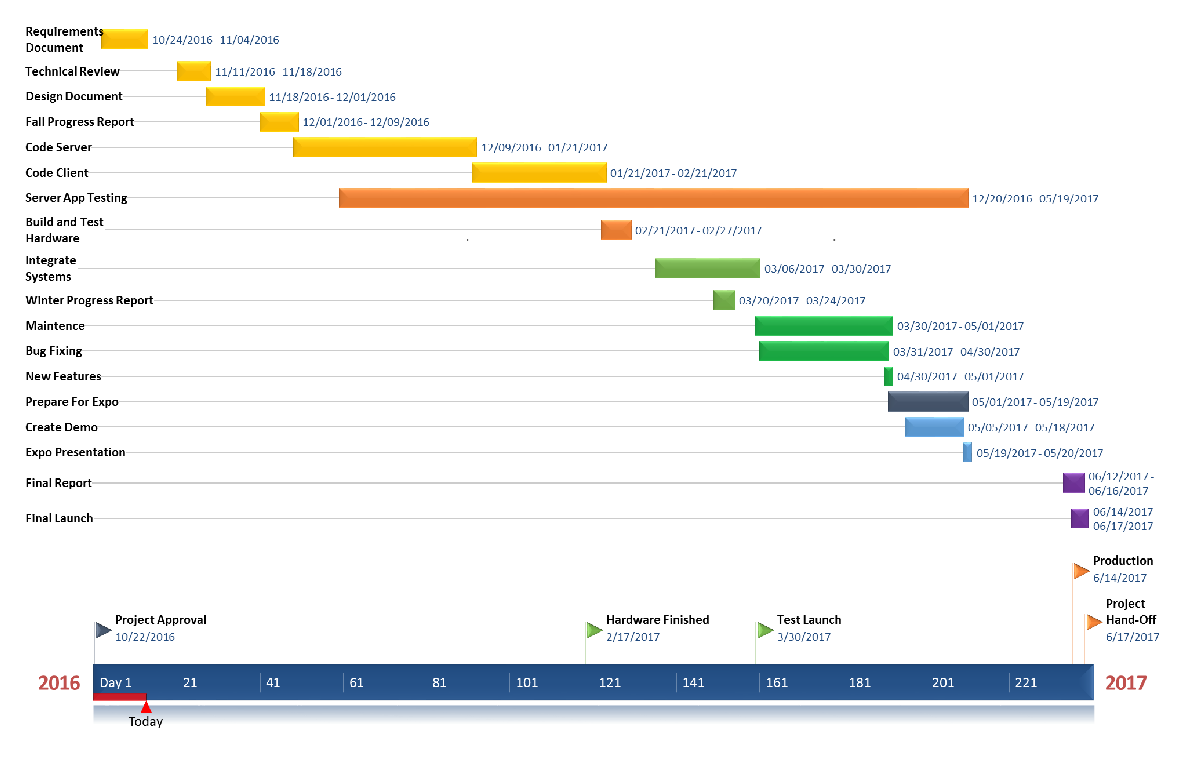
\includegraphics[width=\linewidth]{ganttchart.eps}
  \caption{A Gantt, or timeline, Chart for the 100k rocketry software team.}
  \label{fig:gantt}
\end{figure}

Figure \ref{fig:gantt} shows a gantt chart.

\begin{minipage}{\textwidth}
	
	\vspace{1in}
	\noindent Nancy Squires

	\vspace{1in}
	\noindent Natasha Anisimova

	\vspace{1in}
	\noindent Terrance Lee

	\vspace{1in}
	\noindent Albert Morgan\\

\end{minipage}




\end{document}


